\scanpage{105}
\mspage{7}
the boundary \deleted{\unsure{x}} $S_i=\dot{D}_{i+1}$ of $D_{i+1}$, more specifically these images are just two ``complementary'' hemispheres in $S_i$, which I will denote by $S_i^+$ and $S_i^-$. The kernel of the pair $({\unsure{\phi|\delta|\varnothing}}_i^+,\phi_i^-)$ is just $S_{i-1}=\mathring{D}_i$, and the common restriction of the maps $\phi_i^+,\phi_i^-$ to $S_{i-1}$ is an isomorphism
\[
\deleted{\unsure{on}}\qquad S_{i-1}\simeq S_i^+\cap S_i^-.
\]
This $S_{i-1}$ in turn decomposes into the two hemispheres $S_{i-1}^+$, $S_{i-1}^-$, images of $D_{i-1}$. Replacing $D_{i+1}$ by $D_{\deleted{i}\handwritten{n}}$, we see that the $\deleted{i}\handwritten{n}$-cell $D_{\deleted{i}\handwritten{n}}$ is decomposed into a union of $2\deleted{i}\handwritten{n}+1$ closed cells, one being $D_{\deleted{i}\handwritten{n}}$ itself, the others being canonically isomorphic to the cells $S_j^+,S_j^-$ $\handwritten{(0\leq}j\handwritten{\leq n-1)}$ images of $D_j\to D_n$ by the it\deleted{\unsure{t}}erated morphisms
\[
\phi_{n,j}^+,\,\phi_{n,j}^-:D_j\rightrightarrows D_n.
\]
This is a cellular decomposition, corresponding to a partition of $D_n$ into $2n+1$ open cells $\mathring{D}_n$, $\mathring{S}_j^+=\deleted{\mathrm{Im}}\phi_{n,j}^+(\mathring{D}_j)$, $\mathring{S}_j^-=\phi_{n,j}^-(\mathring{D}_j)$. For any cell \inserted{in this decomposition,} the incident cells are exactly those of strictly smaller dimension.

When introducing the operation $\overset{n}{*}_\ell$ with $\ell=n-j$, it is seen that this corresponds to cho\deleted{\unsure{a}}osing a map
\[
D_n\longrightarrow(D_n,S_j^+)\amalg_{D_j}(D_n,S_j^-),
\]
satisfying a certain condition \deleted{\unsure{x}}, expressing the formulas I wrote down yesterday for $s_1$ and $t_1$ of $u*_\ell v$ \deleted{\unsure{and}} - the \deleted{\unsure{conditions}} formulas translate into demanding that the restriction of the \unsure{looked(-for|looked-for} map of $D_n$ to its boundary $S_{n-1}$ should be a given map (given at any rate, for $\ell\geq2$, in terms of the operation $*_{\ell-1}$, \deleted{\unsure{it seems|it seemed} \illegible{1}} which explains the point I made that the $*_\ell$-structure is of order just above the $*_{\ell-1}$ structure, namely (inductively) is of order $\ell\ldots$). That the extension of this map of $S_{n-1}$ to $D_n$ does indeed exist, comes from the fact that the amalgamated sum on the right hand side is contractible for obvious reasons.

This gives a clue of what we should call ``standart'' amalgamated sums of the cells $D_i$. The first idea that comes to mind is that we should insist that the space considered should be contractible, excluding amalgamated sums therefore such as
\figure{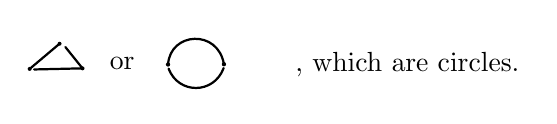
\begin{tikzpicture}[x=1em,y=1em,line cap=round,line join=round]
\draw[thick] (0,0) -- (1.08,.91);
\draw[thick] (1.29,.79) -- (1.91,.02) -- (.16,-.02);
\fill (0,0) circle (.072) (1.08,.91) circle (.072) (1.91,.02) circle (.072);
\node at (3.34,.18) {\handwritten{or}};
\draw[thick] (5,.16) .. controls (5.08,1.34) and (6.80,1.45) .. (7.02,.17);
\draw[thick] (5.02,.01) .. controls (5.37,-.92) and (6.65,-.93) .. (7.01,.03);
\fill (5,.16) circle (.078) (7.02,.17) circle (.078);
\node[anchor=west] at (9.25,.15) {\handwritten{, which are circles.}};
\end{tikzpicture}}
This \deleted{restriction}\inserted{formulation} however has the unconvenience of not being directly expressed in combinatorial terms. The following formulation, which has the advantage of being of combinatorial nature, is presumably equivalent to the former, and gives \deleted{\unsure{enough}} (I expect) \deleted{enough} a large enough notion of ``standartness'' to yield \deleted{\unsure{f}}\unsure{fpr|for} the corresponding notion of $\infty$-category \unsure{enough structure for whatever one will ever need.} \unsure{In any case, it is}
% archive sheet number: 104
